%%% Frontiers in Artificial Intelligence — Original Research
%%% Uses the Frontiers Harvard (author-date) template (FrontiersinHarvard.cls).
%%% Compile: pdflatex; bibtex; pdflatex; pdflatex  (Frontiers-Harvard.bst + references.bib)

\documentclass[utf8]{FrontiersinHarvard}
\usepackage{url,hyperref,lineno,microtype,subcaption}
\usepackage{booktabs}
\usepackage{array}
\usepackage{calc}
\usepackage{longtable}
\usepackage[singlespacing]{setspace}
\linenumbers
\raggedbottom

\def\keyFont{\fontsize{8}{11}\helveticabold }
\def\firstAuthorLast{Chincholikar {and} Chawla}
\def\Authors{Samir Chincholikar\,$^{1}$, Robin Chawla\,$^{2,*}$}
\def\Address{$^{1}$Independent Researcher, New York, NY, United States \\ $^{2}$Independent Researcher, New York, NY, United States}
\def\corrAuthor{Robin Chawla}
\def\corrEmail{robin.chawla.cse14@iitbhu.ac.in}

\begin{document}
\onecolumn
\firstpage{1}

\title[The AI Incident Disclosure Shadow]{The AI Incident Disclosure Shadow: An Incident-Level Study Matching AIID-Recorded AI Failures to U.S.-Listed Companies' Investor Disclosures, 2019--2026}

\author[\firstAuthorLast ]{\Authors}
\address{}
\correspondance{}
\extraAuth{}

\maketitle

\begin{abstract}
\section{}
Publicly traded companies are increasingly developing and deploying artificial intelligence (AI) systems, and there is a growing public record of incidents in which those systems have caused or contributed to real-world harms. But whether they are subsequently reported to investors through securities filings has not been systematically measured. This study connects all incidents in the AI Incident Database (AIID) from 2019--2026 (n = 1{,}389) to organizations identified as developers or deployers of the systems in question. Incidents involving U.S.-listed issuers filing domestic periodic reports result in an analytical sample of 307 incidents spanning 21 issuers. For each incident, we analyze the Forms 8-K, 10-K, and 10-Q filed within the subsequent 12 months and classify them into four levels of disclosure: incident-specific disclosure (T1), legal-proceedings-only disclosure (T2), generic risk disclosure on the same technology or harm, but without reference to the incident (T3), or no related disclosure (T4). Only 4 of 307 incidents received incident-specific disclosure (1.3\%; Clopper--Pearson 95\% CI, 0.4--3.3), and 7 of 307 incidents received either incident-specific or legal-consequence disclosure (2.3\%; 95\% CI, 0.9--4.6). The remaining 97.7\% (95\% CI: 95.4--99.1) constitutes what we refer to as the AI incident disclosure shadow, with 278 incidents (90.6\%) associated with generic risk language but no incident-specific disclosure. We find no detectable association between substantive disclosure and incident severity (Monte Carlo exact p = 0.61), but there are differences depending on whether the issuer is named as the system's deployer or developer (exact p = 0.02). Results are robust to alternative disclosure windows, issuer-concentration checks, and an independent full-filing audit of 40 incidents finds no missed substantive disclosures. The seven incidents that were substantively disclosed are concentrated among cases with financial-statement or formal legal consequences, including two that came with booked charges of approximately \$304 million and \$478 million. These findings document a substantial gap between publicly reported AI incidents and incident-specific investor disclosure. The study measures disclosure incidence, not legal compliance, and provides an incident-level baseline to assess changes in corporate AI transparency.

\tiny
\keyFont{ \section{Keywords:} artificial intelligence incidents, securities disclosure, SEC filings, AI governance, corporate transparency, materiality, risk disclosure }

\keyFont{ \section{Word count:} $\approx$7000 (main text, per Frontiers' definition); Figures: 4; Tables: 4 }
\end{abstract}

\section{Introduction}

Artificial intelligence (AI) systems are increasingly embedded in products, services, operational processes, and financial decision-making. AI's growing economic relevance and the increasing dependence of firms on algorithmic systems have been illustrated by research that documented the expanding role of AI in financial-market prediction, portfolio management, automated financial services, and auditing. At the same time, AI deployment can result in operational, legal, reputational and financial harms when systems perform unexpectedly, produce inaccurate outputs, discriminate among users or contribute to other adverse outcomes. As the economic importance of these systems grows, a critical capital markets question arises: When a publicly traded company is implicated in a reported AI incident, does that incident appear in the information provided to investors?

This question is different from the wider literature on the effect of AI on financial performance, forecasting, investment decisions or organizational efficiency. Previous research has largely focused on using AI to improve financial prediction, portfolio allocation, advisory services, and audit processes. Much less is known about the reverse information channel, namely how firms communicate the adverse consequences of their own development or deployment of AI to capital-market participants. The increasing availability of public incident repositories enables the monitoring of AI-related failures independent of corporate securities filings. This creates an opportunity to compare an external record of incidents with the information that firms disclose to investors.

This study fills the gap at the incident level. We link incidents reported in the AI Incident Database (AIID) from 2019 to 2026 to U.S.-listed companies identified as developers or deployers of the systems in question. We then look at Forms 8-K, 10-K and 10-Q filed during the 12 months following each incident. Rather than a binary outcome, we distinguish four observable disclosure states: incident-specific disclosure (T1), disclosure of a related legal or regulatory consequence without specifically identifying the underlying AI incident (T2), generic risk language describing the same technology or harm family without identifying the event (T3), and no related disclosure found (T4). This structure enables us to separate incident-specific investor communication from the much broader corpus of generic corporate risk language.

In the absence of an incident-specific disclosure or disclosure of a directly related legal consequence in the relevant securities filings, we describe such incidents as falling within the \textbf{AI incident disclosure shadow}. Importantly, the concept is descriptive rather than legal. The fact that an incident is included in AIID does not imply that the incident was material under securities law, that there was a disclosure obligation or that an issuer failed to comply with a legal obligation. The study therefore asks an empirical disclosure-incidence question: conditional on an externally documented AI incident involving a U.S.-listed issuer, how frequently is that event identifiable in subsequent investor disclosures?

The analysis is based on three expectations. First, if securities disclosure operates through a materiality gate rather than a full incident-reporting system, incident-specific disclosure should be rare relative to the number of publicly documented AI incidents (\textbf{H1}). Second, substantive disclosure should be more concentrated among incidents associated with observable financial-statement effects or formal legal and regulatory consequences (\textbf{H2}). This hypothesis refers to an empirical association and does not assume that either channel causes disclosure individually. Third, if the public's perception of harm severity alone is insufficient to determine whether an incident exceeds the firm's disclosure threshold, then substantive disclosure does not need to increase monotonically with incident severity (\textbf{H3}).

This study makes several contributions. First, it provides an incident-level measure of the association between externally recorded AI failures and subsequent securities disclosure. Second, the four-tier taxonomy distinguishes incident-specific disclosure from legal-consequence disclosure, generic coverage of same-family risks, and full non-detection --- avoiding a dichotomous classification that would equate materially different disclosure patterns. Third, the analysis examines whether substantive disclosure (or lack thereof) varies by incident severity and whether the company was a developer or deployer. Separately, the financial and legal characteristics of the small number of substantively disclosed cases are analyzed. Finally, the study stresses reproducibility based on a documented entity-matching process, filing-level search records, independent reliability checks, robustness tests, a hashed pre-analysis plan and an archived replication package. Together, these features provide a baseline against which one can assess how corporate communication on AI incidents might evolve as AI governance and incident-reporting regimes develop.

\section{Related work}

\textbf{AI in the firm and capital markets.} There is a rapidly growing literature on the adoption of artificial intelligence by firms, and its implications for financial decision-making and capital markets. Recent studies in this journal include AI-based stock-price forecasting \citep{Rohan2026}, reinforcement-learning approaches to portfolio management \citep{YangPortfolio2026}, the adoption of automated and hybrid robo advisory services \citep{Verma2026}, and the use of AI to improve the quality of audit and reduce costs in banking and financial services \citep{Johri2026}. Related work associates corporate AI adoption with outcomes such as ESG performance, stock-price crash risk \citep{Shen2025,YangCrash2026}, and, in governance literature, develops frameworks for responsible AI adoption and risk management \citep{Madanchian2025}. Cumulatively, this literature indicates that AI is becoming more economically relevant but it largely discusses adoption, performance, efficiency and governance. It provides relatively little evidence of what happens to investor disclosure after a documented adverse event involving an AI system. We address this downside information channel directly.

\textbf{Regulation of materiality and disclosure.} Securities disclosure is not a complete incident reporting system. The disclosure of information is partly related to materiality, which has traditionally been defined in terms of whether there is a substantial likelihood that a reasonable investor would consider the information important, with contingent events being assessed in terms of both probability and magnitude \citep{TSC1976,Basic1988}. Empirical evidence also demonstrates that disclosure mandates operate within broader institutional and enforcement environments, and can have meaningful impacts on corporate reporting behavior \citep{ChristensenHailLeuz2016,LeuzWysocki2016}. These principles motivate an important distinction for the present study: an external observation of an AI incident does not establish that disclosure of the incident was required under securities law. We thus assess whether the reported incidents are mentioned in later filings, without making legal determinations about specific issuers or events.

\textbf{Voluntary disclosure and risk factor text.} The existing literature indicates that disclosures of corporate risk factors convey information that investors find relevant \citep{Campbell2014,KravetMuslu2013} and that more specific disclosures are more informative than generalized disclosures \citep{Hope2016}. More generally, the filings-text literature shows how text analysis can be used to identify and classify corporate risks at scale \citep{LoughranMcDonald2011,BaoDatta2014}. The voluntary-disclosure theory provides an alternative explanation of why firms might not disclose all adverse information. Classical models predict incentives for more disclosure \citep{Grossman1981,Milgrom1981}, but proprietary costs, reputational concerns, uncertainty and managerial incentives may interrupt this process \citep{Dye1985,Verrecchia2001,HealyPalepu2001}. Also, empirical evidence indicates that managers may selectively disclose bad news or delay the disclosure of bad news \citep{Skinner1994,KothariShuWysocki2009,Beyer2010}. We add to this literature by relating it to realized AI incidents. We differentiate between incident-specific disclosure and generic risk language that refers to the same technology or harm category, but without naming the underlying event.

\textbf{Cybersecurity disclosure: the closest analog.} The closest empirical analogy is cybersecurity disclosure. Prior studies have documented publicly observable cybersecurity events preceding corporate disclosures, showing market impacts of announced breaches and disparities between actual cybersecurity events and cyber risk disclosures in securities filings \citep{Campbell2003,KannanReesSridhar2007,Gordon2006,Gordon2010,WangKannanUlmer2013}. Other work finds evidence that cyber-attacks can be under-reported in relation to events observable through other information channels \citep{Amir2018}. The conceptual parallel is important: both cybersecurity and AI generate operational events that could be publicly visible outside the issuer's own reporting system. We adopt this design for AI by constructing an incident-level denominator using an external incident database, then examine the ability to identify each matched event in subsequent investor filings.

\textbf{AI harms, audits and incident reporting.} Another set of literatures detail taxonomies of AI harms and frameworks for auditing artificial intelligence systems \citep{Weidinger2022,Raji2020,Bommasani2021,CostanzaChock2022}, and incident repositories such as AIID and related classification efforts have cataloged harms that have already occurred \citep{McGregor2021,OECD2024}. Further research in other safety-critical domains has shown that recorded incident rates can be significantly driven by reporting incentives, institutional design and the availability of confidential or non-punitive reporting channels \citep{Barach2000,Classen2011,Macrae2016}. These literatures emphasize the significance of documenting realized harms, but they do not answer whether externally recorded AI incidents subsequently become visible to investors. We directly measure that connection by matching incident records to issuer filings and differentiate between incident-specific communication, disclosure of related legal consequences, generic same-family risk coverage, and cases in which no related disclosure is found.

\section{Materials and methods}

\subsection{Study design and universe of incidents}
The study uses an incident-level design that links externally documented AI incidents to subsequent securities disclosures by U.S.-listed companies. The incident universe is taken from a full snapshot of the AI Incident Database (AIID) as of 27 July 2026. The archived source file contains 1{,}597 incident records, of which 1{,}389 have incident dates between 2019 and 2026 and thus constitute the initial study population. We kept the source snapshot with a SHA-256 hash so that the underlying incident universe can be verified independently.

The unit of analysis is the single AI incident. Each AIID record was reviewed to identify the organization(s) described as developing, deploying, operating, or otherwise directly associated with the AI system in question. Then, organizations were aligned to publicly-listed issuers and where needed, resolved to corporate parents. If at least one of the implicated organizations could be linked to a U.S.-listed domestic issuer that files periodic reports with the U.S. Securities and Exchange Commission (SEC), the incident was included in the analytical sample.

The procedure resulted in 307 matched incidents for 21 issuers (Figure~\ref{fig:flow}). The remaining AIID incidents were excluded because they involved private companies (n = 243), organizations that could not be resolved with sufficient confidence (n = 400), generic or individual actors rather than identifiable firms (n = 398), foreign-listed issuers that fell outside the study's scope (n = 26), or companies that had been delisted during the relevant period (n = 15). The matched sample is concentrated at a handful of large technology firms: Alphabet accounted for 86 incidents, Meta for 81, Tesla for 36, and Microsoft for 35. The issuer-level Herfindahl--Hirschman Index was 0.18. The robustness analysis explicitly accounts for issuer concentration, which may affect estimates at the incident level.

\subsection{Entity resolution and issuer matching}
The entity resolution process began with the organizations named in each AIID incident and progressed to the corresponding publicly listed corporate entity. When an incident cited a subsidiary, product, platform, or acquired company, the record was linked to the publicly listed parent if it was possible to confirm the ownership relationship with enough confidence for the date of the incident. During matching, we also recorded the issuer's role in the incident --- whether the company was identified as a developer of the AI system, as a deployer or operator, or as both.

To validate recurring organization-to-issuer mappings and corporate-parent relationships, a human-validation crosswalk was constructed with 137 rows. The process identified and corrected two incident-level mapping errors prior to finalizing the analytical dataset. We also examined high-frequency firm names that did not match, to determine whether the matching procedure systematically excluded other U.S.-listed issuers. The audit did not identify any additional issuer that could be added with sufficient confidence.

Therefore, the 307 resulting incidents should be interpreted as the subset of AIID incidents that could be conservatively and reproducibly matched to U.S.-listed domestic issuers under the study protocol. The procedure does not establish that every AIID incident for a listed company was successfully identified, especially where organizational identities or parent relationships were ambiguous.

\subsection{Filing retrieval and disclosure window}
SEC filings were searched beginning on the date of each matched incident and continuing for 12 months. The primary search universe is the Forms 8-K, 10-Q, and 10-K of the matched issuer for that period. The 12-month window was selected to capture both current reports and at least one additional cycle of periodic reporting, while remaining within a consistent incident-centered observation period.

Retrieval of filings was done via the issuer's Central Index Key (CIK) and deterministic filing URLs. Searches used three families of terms to identify (1) the specific system, product, organization or incident described in the AIID, (2) the relevant artificial intelligence technology or application, and (3) the type of harm or consequence associated with the event. Search terms were recorded at the incident level. In the Risk Factors and Legal Proceedings sections, we also reviewed the first annual report following each incident, even if keyword searches did not produce a clear incident-specific match.

Search results were rated in context rather than classified only by keyword occurrence. The candidate passages were read to see if the filing was about the underlying incident, a related legal or regulatory fallout or simply a more general category of technology risk. This distinction is central to the disclosure taxonomy below.

\subsection{Disclosure classification}
Each incident was classified into one of four, mutually exclusive disclosure tiers based on the strongest disclosure that occurred within the observation window.

\textbf{T1 --- Incident-specific disclosure:} disclosure is tied to the AIID incident by identifying the underlying event with sufficient factual specificity. The filing does not need to use the term ``artificial intelligence'' if the event, system, product, or factual circumstances identify the connection.

\textbf{T2 --- Legal-proceedings-only disclosure:} the filing reports a lawsuit, investigation, regulatory proceeding, settlement, contingency, or other formal legal consequence associated with the incident, but does not describe the underlying event as an AI incident with sufficient specificity to qualify as T1.

\textbf{T3 --- Generic risk disclosure:} the issuer discloses the same technology or harm family implicated in the incident in the disclosure window, but does not identify the incident itself or a directly associated legal consequence.

\textbf{T4 --- No related disclosure found:} no incident-specific disclosure, related legal-consequence disclosure, or same-family generic risk language found in the filing universe examined per the protocol.

T1 is the primary measure of incident-specific disclosure. A broader measure of \textbf{substantive disclosure} combines T1 and T2 because both provide investors with information traceable to the event or its formal consequence. \textbf{The AI incident disclosure shadow} is T3+T4. This definition is descriptive: it refers to incidents for which no incident-specific disclosure and no disclosure of a directly related legal consequence could be found. This does not imply that disclosure was legally required.

It is important to distinguish T3 from T4. T3 means the issuer was already discussing the relevant type of artificial intelligence (AI) technology or harm with investors but not the specific incident that occurred. T4 means no similar disclosure was found. We thus view T3 as generic-risk coverage without incident-specific disclosure, rather than as evidence of intentional substitution of generic language for disclosure of the event.

\subsection{Coding procedure and reliability}
In the first pass, all 307 incidents were coded using a pre-specified codebook and decision tree. Each classification was linked to the filing evidence supporting the assigned tier. Filing evidence included filing date, form type, filing location, search terms, and relevant passage where applicable.

A second independent coding pass was performed on a stratified sample of 68 incidents. The reliability sample consisted of all T1 and T2 cases, 21 of 22 T4 cases, and a random sample of 40 T3 cases. This design intentionally oversampled the rare disclosure categories and the cases close to the substantive/non-substantive classification boundary.

Raw agreement, Cohen's kappa \citep{Cohen1960}, prevalence-adjusted and bias-adjusted kappa (PABAK) and Gwet's AC1 \citep{Gwet2008} were used to evaluate agreement. We also calculated an inverse-probability-weighted agreement estimate to approximate agreement across the full incident distribution, considering that the reliability sample was stratified and not proportionally sampled. Discrepancies were noted and reconciled only after the independent coding comparison was completed.

\subsection{Severity of incidents}\label{sec:sev}
The potential relationship between incident severity and substantive disclosure was also examined. For the 40 incidents for which severity information was available via the CSET AI Harm taxonomy, the existing classification was preserved (Supplementary Table~S1). The other incidents were categorized as Severe, Moderate, or Limited based on a pre-specified harm-severity rubric that utilized the reported outcomes of the incident.

The final sample consisted of 42 Severe, 50 Moderate and 215 Limited incidents. Severity is an indicative analytical measure rather than an authoritative or externally validated ranking of harm, as only a subset of incidents had an external CSET classification and the remaining severity assignments were based on the study rubric. Severity was not subject to a full independent second-coding exercise as was the primary disclosure coding; this limitation is taken into account in the interpretation of the severity analysis.

\subsection{Statistical analysis}
The main estimands are the proportions of incident cases classified as T1, T1+T2, T3, T4 and T3+T4. Rare disclosure outcomes are reported using exact Clopper--Pearson confidence intervals \citep{ClopperPearson1934}, and Wilson intervals \citep{Wilson1927} are used where appropriate for complementary descriptive estimates.

At the company level, observations are not assumed to be fully independent, because multiple incidents are associated with the same issuers. Therefore the main incident-level estimates are complemented with a 10,000-resample issuer-clustered bootstrap. The clustered estimates are interpreted with caution (limited number of issuer clusters, 21) and are reported with the exact incident level intervals, not as a replacement for the latter.

Monte Carlo exact permutation tests with 20,000 iterations were used to examine differences in substantive disclosure by severity categories and issuer roles. The asymptotic regression estimates based on the conventional approach are unstable due to sparse outcomes: there are only seven incidents in the sample that are either T1 or T2. Therefore, no confirmatory multivariable logistic model is considered the primary inferential analysis. The severity analysis tests whether the observed distribution of disclosure differs across severity groups. Failure to reject the null is interpreted as the absence of detectable evidence of a severity gradient rather than proof that severity and disclosure are exactly independent.

All statistical analyses were performed using deterministic scripts with a fixed random seed of 42. The final analytical data set was used to independently re-derive the reported statistics, tables and figures.

\subsection{Robustness and retrieval audits}
In several analyses we investigate the sensitivity of the main estimate to a number of design choices made in the study. Alternative 6-, 18-, and 24-month filing windows were used to recalculate disclosure classifications. To address right-censoring near the end of the study window, the analysis was also repeated restricting the sample to incidents with complete follow-up periods.

Issuer concentration was assessed with leave-one-issuer-out analyses and by sequentially excluding the most incident-intensive issuers. These tests take into account whether the overall disclosure shadow is largely an artifact of a small number of companies accounting for a disproportionate share of incidents.

A separate audit of retrievals was performed to determine whether substantive disclosures were missed by the structured filing-search process. Forty incidents (20 T3 and 20 T4) were randomly selected from the non-substantive categories. All relevant filings in the observation window of each selected incident were read in full without relying on the original keyword-search procedure. The audit found no missed T1 or T2 disclosures. With no misses among the 40 audited incidents, the exact one-sided 95\% upper confidence bound on the underlying miss rate is approximately 7.2\%. All seven T1 and T2 classifications were also manually rechecked against the underlying filings.

\subsection{Reproducibility and research workflow}
The analytical workflow was pre-registered through a hashed pre-analysis plan prior to final estimation detailing the core sample construction, disclosure taxonomy, primary estimands, procedures for assessing reliability, and procedures for assessing robustness. The replication package includes the 307-incident matched dataset, disclosure classifications, severity coding, issuer-matching crosswalk, filing-search records, disagreement log, pre-analysis documentation, and analysis code to reproduce the reported tables, figures, and statistical results. The researchers defined the disclosure codebook and classification rules, and all entity matches, filing evidence, incident classifications, and final statistical outputs were validated. Each of the reported disclosure classifications can be traced back to the underlying source filing. The main results were independently re-derived using the final data. A generative-AI system (Anthropic Claude, Opus-class model, accessed August 2026 via the Claude Agent SDK) assisted with software scaffolding and coding of these scripts and with language editing, under author validation; all study design, entity resolution, incident classification, and interpretation were performed by the authors (see the Generative AI Statement).

\section{Results}

\subsection{Primary disclosure outcomes}
The final analytical sample includes 307 AI incidents involving 21 U.S.-listed issuers. Incident-specific disclosure was infrequent (Table~\ref{tab:dist}). Only 4 incidents were classified as T1, corresponding to 1.3\% of the sample (Clopper--Pearson 95\% CI: 0.4--3.3\%). An additional 3 incidents were coded as T2 because while a related legal or regulatory consequence was mentioned in the issuer's filings, the underlying AI incident was not described with sufficient specificity to be coded as T1. Substantive disclosure was reported for 7 of 307 incidents or 2.3\% (95\% CI: 0.9--4.6\%) when combining these categories.

Most events were instead associated with generic risk disclosure. Of these incidents, 278 (90.6\%) were categorized as T3, meaning the issuer disclosed risks associated with the same technology or harm family in the relevant time period without identifying the incident itself. An additional 22 incidents (7.2\%) were classified as T4, for which no related disclosure was identified under the study protocol. In total, T3 and T4 account for 300 of 307 events, yielding an AI incident disclosure shadow of 97.7\% (95\% CI: 95.4--99.1\%). A bootstrap clustered by issuer gave a similar estimate of 97.5\% (95\% CI: 93.9--99.6\%).

The composition of the disclosure shadow is important. The disclosure shadow is driven primarily by generic risk coverage rather than complete disclosure silence. In more than nine out of ten cases, the filing language referred to the relevant class of technology or harm, but the specific incident was not identified. Thus, the main result indicates a substantial difference between disclosure of general AI-related risk and disclosure of realized AI incidents.

\subsection{Incident severity and substantive disclosure}
Furthermore, substantive disclosure did not increase monotonically with the study's severity classification (Table~\ref{tab:sev}). Of the 42 incidents classified as Severe, 2.4\% received T1 disclosure and 4.8\% received either T1 or T2 disclosure, leaving 95.2\% in the disclosure shadow. Among 50 Moderate incidents, none received T1 disclosure, 2.0\% received T1 or T2 disclosure, and 98.0\% remained within the disclosure shadow. Of the 215 Limited incidents, 1.4\% received T1 disclosure, 1.9\% received T1 or T2 disclosure, and 98.1\% remained in the shadow.

A Monte Carlo exact permutation test found no statistically distinguishable distribution of substantive disclosure across the three severity groups (p = 0.61; Figure~\ref{fig:sev}). Thus, the result offers no evidence for a severity gradient in this sample. This should not be taken to mean that incident severity and disclosure are exactly independent, especially given the small number of substantive disclosures and the attendant limits on statistical power.

\subsection{Issuer role and disclosure}
We carried out a pre-specified secondary analysis to evaluate if the involvement of the issuer in the incident was related to disclosure. Substantive disclosure was unequally distributed between the developer and deployer roles (Monte Carlo exact p = 0.02). All four T1 disclosures featured an issuer as a deployer of the implicated system. No incident-specific T1 disclosure was made for any of the 58 developer-only role incidents.

Since only seven incidents are substantive disclosures, these role differences should be interpreted as descriptive evidence rather than as estimates of a stable causal relationship between organizational role and disclosure. The result nevertheless suggests that the position of the issuer in the development and deployment chain may be relevant to whether an incident becomes identifiable in follow-up investor reporting.

\subsection{Characteristics of events with substantive disclosures}
The seven T1 or T2 incidents were concentrated in cases with observable financial-statement effects or formal legal and regulatory consequences (Table~\ref{tab:acct}). Two T1 cases had large booked financial impacts. Zillow said it incurred roughly \$304 million in charges to wind down its algorithm-driven business of buying and selling homes, while General Motors said it incurred roughly \$478 million in restructuring charges to suspend its autonomous-vehicle business.

The remaining substantive matters were primarily litigation, regulatory proceedings, investigations or related contingencies. These included incident-specific disclosures about legal proceedings and T2 cases where the filing described the resulting legal or regulatory matter but did not identify the underlying event as an AI incident. Conversely, two of the largest incident categories in the sample --- misinformation or content-related incidents (n = 70) and generative-AI error incidents (n = 57) --- contained no substantive disclosures.

This concentration is consistent with H2 in a descriptive sense, with substantive disclosures concentrated among incidents associated with recognized financial-statement or formal legal reporting channels. There is no evidence that these consequences led to disclosure and the small number of positive cases does not support a formal mechanism test.

\subsection{Issuer concentration and temporal patterns}
Disclosure of substance was not evenly spread among issuers. Of the 21 issuers in the analytical sample, only 4 had one or more T1 or T2 incidents. At the same time, the relatively high overall disclosure-shadow estimate is not solely driven by the companies contributing the largest numbers of incidents (Table~\ref{tab:rob}; Figure~\ref{fig:pareto}).

In leave-one-issuer-out analysis, the estimated disclosure shadow ranged from 96.8\% to 98.6\%. Removing the two issuers with the most incidents, the shadow estimate fell to 96.4\% and removing the five issuers with the most incidents, the estimate was 92.5\%. Therefore, although issuer concentration does influence the magnitude of the estimate, the key finding is that the large majority of externally recorded incidents could not be identified via incident-specific or related legal-consequence disclosure.

We also tested whether the substantive disclosure increased over the period of the study. No systematic time increase was found. A trend test indicated z = $-0.28$ (p = 0.78; Figure~\ref{fig:year}), providing no evidence that the probability of substantive disclosure increased across incident years represented in the sample.

\subsection{Coding reliability and retrieval validation}
Independent second-coding exercise indicated an agreement of 85.3\% on the raw agreement across the stratified reliability sample. The Cohen's kappa was 0.73, the prevalence-adjusted and bias-adjusted kappa was 0.71 and the Gwet's AC1 was 0.82. The inverse-probability-weighted agreement estimate was 90.9\% (adjusted for intentional oversampling of rare disclosure categories).

In the reliability sample, 10 disagreements were found between coders. Four crossed the main substantive/non-substantive divide separating T1 or T2 from T3 or T4. The remainder of the disagreements concerned distinctions within these larger groups. The results indicate substantial agreement, but also show that judgment is needed for classification near the boundary between legal-consequence disclosure and generic risk language.

The separate retrieval audit was a further check on the filing-search procedure. All relevant filings for 40 randomly selected non-substantive incidents (20 T3 and 20 T4 cases) were read in full and without searching. No previously missed T1 or T2 disclosures were found. The exact one-sided 95\% upper confidence bound on the underlying miss rate is approximately 7.2\%, with no misses among 40 audited incidents. All seven substantive disclosure cases were manually re-audited using the underlying filings.

\subsection{Robustness to alternative specifications}
The primary outcome is stable in comparison to other design choices (Table~\ref{tab:rob}). Re-estimating disclosure outcomes with 6-, 18-, and 24-month filing windows did not materially alter the finding that substantive disclosure was rare and that the large majority of incidents remained in the disclosure shadow. Similarly, restricting the analysis to those incidents with complete follow-up periods also yielded similar results, suggesting that right-censoring close to the end of the study period does not explain the primary estimate.

All of the alternative windows, issuer-concentration analyses, complete-follow-up restriction, independent coding exercise, and full-filing retrieval audit point to the same empirical pattern: disclosure of incident-specific or directly related legal consequences is not common among AIID incidents matched to U.S.-listed issuers, while generic same-family risk disclosure is common.

\section{Discussion}

This study provides incident-level evidence on whether publicly documented AI failures involving U.S.-listed companies subsequently become identifiable in securities filings. Of the 307 AI incidents by 21 issuers, only four incidents had incident-specific disclosure, and only seven had incident-specific disclosure or disclosure of legal consequence that was directly related to the incident. The resulting coverage of the AI incident disclosure shadow is 97.7\% of the sample. Thus, the main finding is not that incident-specific disclosure is rare, but that realized AI incidents and investor-facing disclosure often occupy different informational layers.

The composition of this shadow is especially revealing. Most incidents were classified as T3 rather than T4. Specifically, 278 of 307 incidents were associated with filing language addressing the same technology or harm family without identifying the particular incident. Complete absence of related disclosure was less common by a wide margin. This pattern should not be viewed as evidence that issuers intentionally substituted disclosure of a particular event with generic language. The data do not reveal managerial intent, nor do they prove that generic language was written in response to an incident. Instead, they point to a narrower empirical result: general coverage of AI-related risks is ubiquitous, even if the realized incidents remain individually unidentified in those filings.

This distinction helps to clarify the relationship between risk disclosure and actual events. Incident disclosure is retrospective, pertaining to a specific event that has occurred, whereas risk-factor reporting is generally prospective and categorical. So a filing can acknowledge that a class of AI-related harm may exist without identifying every instance in that class. The results show that this difference is not small in the current sample; it accounts for the vast majority of observed incidents. Therefore, corporate AI transparency research focusing on whether firms disclose AI-related risks may substantially overstate investors' ability to detect actual negative consequences from such disclosures.

The seven substantively disclosed cases shed more light on what situations make an AI incident visible in investor reporting. These cases are concentrated in incidents with financial statement effects or formal legal or regulatory consequences. Two incident-specific cases had associated booked charges of approximately \$304 million and \$478 million, while several others emerged through litigation, regulatory proceedings, investigations or related contingencies. By contrast, large categories of misinformation, content-related harms, and generative-AI errors produced no substantive disclosures in the study sample.

This pattern fits H2. The evidence supports an association, although not an identified mechanism. The study cannot tell if an issuer disclosed an incident in response to accounting recognition or legal proceedings. The T2 category is also characterized by the existence of a formal legal consequence in the filing, and so the legal component of this pattern should not be viewed as an independent causal test. The more persuasive evidence is the wider spread of positive cases around incidents that made their way into established financial-reporting or legal-reporting channels, including the two T1 cases with large booked charges. To test these channels independently would require a larger sample and more substantive disclosures.

The severity results further complicate a simple model in which more harmful AI incidents are necessarily more visible to investors. Substantive disclosure was present in 4.8\% of Severe incidents, 2.0\% of Moderate incidents, and 1.9\% of Limited incidents, but the exact test did not find the difference to be statistically distinguishable (p = 0.61). This result is consistent with H3 in the limited sense that the study does not find a monotonic severity gradient. It does not prove that severity has no bearing on disclosure. We observe only seven substantively meaningful disclosures, which severely limits the statistical power. The severity measure itself combines externally available classifications with a study-specific rubric. The result is better interpreted as indicating that the severity of observable harm alone does not clearly explain what incidents become identifiable in securities filings.

The secondary analysis on issuer role gives a different pattern. Disclosure differs for developer versus deployer (exact p = 0.02) and all four incident-specific T1 disclosures are by issuers as deployers. None of the 58 developer-only incidents got T1 disclosure. One interpretation is that firms are more likely to suffer recognizable operational, accounting or legal consequences when they directly deploy an AI system than when they only are involved in its development. However, the current data do not isolate that mechanism and the small number of positive cases makes the result more appropriate as a hypothesis-generating finding than as a stable estimate of role effects.

The results are consistent with a materiality-gated disclosure setting. Securities filings are not intended to be a complete repository of every operational incident related to a public company. An externally reported AI incident may be publicly salient without necessarily resulting in a financial impact, legal proceeding, or other consequence that results in identifiable investor disclosure. Meanwhile, the absence of incident-specific disclosure means that investors who rely on periodic and current reports would not be able to reconstruct anything like the external incident record represented in AIID.

This has implications for the research on corporate AI transparency. Recent finance research has largely focused on AI as a productive technology for improving financial-market prediction, portfolio management, automated financial services, and auditing. In the present study, the information flow is looked at in the reverse direction. Instead of asking how AI improves financial decisions, it asks what investors learn when artificial intelligence systems themselves are the source of an adverse event. The results indicate that this downside information channel is much narrower than the broader corporate discourse on AI-related risk.

The robustness checks further support the main descriptive finding. Even when issuers with the most incidents are excluded, and even when alternative 6-, 18-, and 24-month disclosure windows are used, and even when the analysis is restricted to incidents with a full follow-up period, the disclosure shadow remains large. Leave-one-issuer-out estimates range from 96.8\% to 98.6\%, and removal of the five largest incident contributors still produces a shadow estimate of 92.5\%. The results suggest that the main finding is not an artifact of a single issuer, a single observation window, or right-censoring toward the end of the sample period.

The independent coding and retrieval exercises, which also highlight areas of uncertainty, provide further support. The second coding pass revealed a high level of agreement on many reliability statistics; however, four disagreements crossed the substantive/non-substantive divide. The full-filing audit of 40 randomly selected T3 and T4 incidents identified no missed substantive disclosure. However, observing zero misses in 40 does not mean that the miss rate is zero. The one-sided 95\% upper confidence bound is about 7.2\%. Hence the retrieval audit supports the search protocol without precluding the possibility that some obliquely worded disclosures are still missed.

The results provide a useful baseline to compare future results against. Researchers can examine whether the relationship between externally reported incidents and investor-facing disclosure changes as AI-specific governance and incident-reporting systems are developed. Current estimates describe a period in which the frequency of AI incidents was high enough to generate a large external record, but incident-specific securities disclosure was still rare. Repeating the same incident level design under future reporting regimes allows us to separate changes in general AI risk discussion from changes in the disclosure of realized events themselves.

Most importantly, the AI incident disclosure shadow should not be seen as a sign of unlawful nondisclosure. This study does not make any determination as to whether any particular incident was legally material, whether an issuer had a duty to disclose it, or whether an issuer complied with applicable securities law. The contribution is empirical rather than adjudicative: for AI incidents independently recorded in AIID and matched to U.S.-listed issuers, a small minority became identifiable via incident-specific or directly related legal-consequence disclosure. This gap between the external incident record and investor-facing filings is the phenomenon documented here.

\section{Limitations}

There are some limitations to this study that should be taken into account when interpreting the results. First, the AI Incident Database is not a census of all AI-related failures. It is a media-derived repository. The database is biased toward events that have been made public, while internal events, events with limited media coverage, or events that cannot easily be attributed to a specific organization might be absent. Therefore, the analytical sample represents externally documented and matchable incidents rather than the total population of AI failures involving publicly listed companies. The estimated disclosure shadow should not be interpreted as a formal lower bound since the disclosure behavior of unrecorded incidents is unobservable.

Second, issuer matching necessarily involves judgment. During the study period, 1{,}389 AIID incidents were identified, of which 307 could be matched conservatively to 21 U.S.-listed domestic issuers. Many records had unresolved organizational identities, uncertain relationships between developers, deployers, subsidiaries, and parent companies, or entities outside the scope of the study. We tried to minimize mapping error through the use of a 137-row validation crosswalk and an additional audit of frequently occurring unresolved organizations, but it is possible that some eligible incidents were missed. The denominator generated should thus be understood as the reproducibly matchable sample generated by the study protocol rather than an exhaustive census of listed-company AI incidents.

Third, the matched sample is concentrated in a relatively small number of technology companies. Alphabet, Meta, Tesla and Microsoft account for a large share of the observations and only 21 issuers are represented in total. Leave-one-issuer-out analyses, sequential exclusion of the largest incident contributors and issuer-clustered bootstrap estimates suggest these firms are not the sole drivers of the main result. However, the small number of issuer clusters limits statistical inference and the extent to which the estimated disclosure rate can be generalized to the wider population of U.S.-listed companies.

Fourth, there are still measurement errors in filing retrieval. The language used to describe AI-related events varies greatly in media reports, corporate filings, legal proceedings and product documentation. The search protocol included incident-specific, technology-related and harm-related terms, and manual review of relevant sections of filings, but unusually indirect or oblique disclosures may have been missed. The independent full-filing audit of 40 randomly selected T3 and T4 incidents did not find any missed substantive disclosures. This provides support for the retrieval procedure. However, zero observed misses in 40 cases yields a one-sided 95\% upper confidence bound of approximately 7.2\%, so the audit cannot prove perfect retrieval sensitivity.

Fifth, the classification of disclosure involves an unavoidable element of judgment, especially at the boundary between disclosure of a legal consequence and general discussion of the same risk. There was substantial agreement in the independent second-coding exercise, but four disagreements crossed the primary substantive/non-substantive boundary. The full sample contains only seven substantive disclosures, so even a small number of classification differences can be proportionately important. Double coding of the entire sample would provide an even stronger reliability assessment.

Sixth, the severity analysis is more exploratory than the main disclosure analysis. External CSET severity information was available for only 40 of the 307 incidents. The remaining observations were classified using a pre-specified study rubric. Severity coding was not independently double-coded in the same manner as the primary disclosure outcome. Therefore, the lack of a statistically discernible severity gradient should be viewed with caution, especially as the limited power to distinguish differences across severity categories is driven by the small number of substantive disclosures.

Seventh, the 12-month disclosure window is a choice of research design, not a theoretically unique interval. Some consequences of AI incidents may be fast developing. Litigation, regulatory investigations, accounting effects or organizational responses may develop over substantially longer periods. The same general conclusion holds for 6-, 18-, and 24-month windows, but there is no fixed observation window that can capture all the possible pathways of disclosure.

Finally, the number of substantive disclosures is limited, which constrains the analysis of mechanisms. Only seven T1 or T2 cases would result in unstable and potentially misleading multivariable models. The concentration of disclosure among incidents with financial-statement effects or formal legal consequences is thus descriptive and should not be construed as causal evidence that these channels independently generate disclosure.

Future research could build on this design by using larger incident populations, more public-company jurisdictions, and longer observation periods. More positive disclosure cases would allow issuer-clustered multivariable modeling of the factors associated with disclosure. Another way to look at whether AI-related incidents that are reported externally but not disclosed have information of value to investors is to connect incidents to market reactions. Cross-jurisdictional comparisons, such as those in jurisdictions with mandatory AI-incident reporting requirements, could also serve as a basis for evaluating whether new reporting regimes change the connection between realized AI harms and investor-facing disclosure.

\section{Conclusion}

This study measures the extent to which publicly documented AI incidents involving U.S.-listed companies become identifiable in subsequent securities filings. Among 307 AIID incidents associated with 21 issuers, only four received incident-specific disclosure and only seven received either incident-specific disclosure or disclosure of a directly related legal consequence. The resulting AI incident disclosure shadow encompasses 97.7\% of the sample.

The dominant pattern is not complete silence. Most incidents were accompanied by generic filing language addressing the same technology or harm family without identifying the realized event. This distinction matters because the presence of broad AI-risk disclosure does not necessarily provide investors with information about specific incidents that have already occurred. The findings therefore reveal a substantial separation between the external record of realized AI harms and the incident-level information observable in investor-facing filings.

Substantive disclosures were concentrated among a small number of incidents associated with financial-statement effects or formal legal and regulatory consequences, including two cases accompanied by substantial booked charges. By contrast, the analysis does not detect a clear relationship between the study's measure of incident severity and substantive disclosure. These patterns are consistent with a disclosure environment in which recognized financial and legal consequences may be more closely connected to investor reporting than publicly observable harm severity alone, although the small number of positive cases prevents causal identification of these mechanisms.

The principal finding remains stable across alternative disclosure windows, issuer-concentration analyses, complete-follow-up restrictions, independent coding checks, and a search-independent full-filing audit. At the same time, the study is bounded by the media-derived nature of AIID, a relatively concentrated issuer sample, uncertainty in entity resolution and severity classification, and the possibility of missed or obliquely worded disclosures.

The AI incident disclosure shadow is a descriptive measure, not a determination of legal materiality or compliance. The study does not establish that any particular incident was required to be disclosed or that any issuer violated a disclosure obligation. Instead, it provides an incident-level baseline showing that, during the study period, only a small fraction of externally documented AI incidents involving U.S.-listed companies became specifically identifiable in securities filings. As AI governance and incident-reporting regimes evolve, this framework provides a reproducible basis for measuring whether realized AI harms become more visible to investors.

\section*{Conflict of Interest Statement}
The authors declare that the research was conducted in the absence of any commercial or financial relationships that could be construed as a potential conflict of interest.

\section*{Author Contributions}
SC: Conceptualization, Methodology, Software, Data curation, Formal analysis, Writing -- original draft. RC: Conceptualization, Validation, Writing -- review \& editing, Supervision. Both authors approved the final version.

\section*{Funding}
This research received no external funding.

\section*{Generative AI Statement}
The authors declare that a generative-AI system (Anthropic Claude, Opus-class model, accessed August 2026 via the Claude Agent SDK) was used to assist with software scaffolding and coding of the analysis pipeline and with language editing and drafting of the manuscript, in all cases under the authors' direction (see also Materials and Methods and the Acknowledgments). It was not used for the study design, data analysis, or interpretation of the results, and the authors take full responsibility for all content. No generative-AI system is listed as an author.

\section*{Acknowledgments}
Software scaffolding and coding of the analysis and verification pipeline, and language editing of the manuscript, were assisted by a generative-AI system (Anthropic Claude, Opus-class model, accessed August 2026 via the Claude Agent SDK) under author validation; see the Generative AI Statement. The corresponding author is responsible for the accuracy of all content, citations, and references.

\section*{Ethics Statement}
This study did not involve human participants or animals. It uses only publicly available records (the AI Incident Database and SEC EDGAR). The study measures disclosure behavior in the aggregate and makes no assertion that any named issuer violated a disclosure duty.

\section*{Data Availability Statement}
All data and code required to reproduce the study are openly available in a published, deterministic computational capsule on Code Ocean \citep{Capsule2026} (\url{https://doi.org/10.24433/CO.2340354.v2}; MIT and CC0). Within the capsule, the dataset is in the \texttt{/data} directory --- the primary file \texttt{data/disclosure\_coding.csv} holds the 307 matched incidents with their four-tier disclosure codes and severity, alongside the incident-to-issuer match table, the per-incident search records and coding logs, the independent-coding disagreement log, and the hashed pre-registration; the analysis and verification scripts are in \texttt{/code} and pre-computed outputs in \texttt{/results}. The capsule reproduces every reported number, table, and figure offline. The source repository (\url{https://github.com/samirrc2/ai-incident-disclosure-shadow}) will be made public upon acceptance. The underlying AIID snapshot is publicly available from the Responsible AI Collaborative; the pinned version and its SHA-256 are recorded in the manifest.

\bibliographystyle{Frontiers-Harvard}
\bibliography{references}

%%%%%%%%%%%%%%%%%%%%%%%%%%%%%%%%%%%%%%%%%%%%%%%%%  TABLES (Frontiers: at end)  %%%%%%%%%%%%%%%%%%%%%%%%%%%%%%%%%%%%%%%%%%%%%%%%%

\begin{table}[h!]
\caption{Four-tier disclosure distribution (N = 307). Intervals are Clopper--Pearson exact 95\%.}
\label{tab:dist}
\centering
\begin{tabular}{@{}llrl@{}}
\toprule
Tier & Meaning & n & Share (95\% CI) \\ \midrule
T1 & Disclosed-specific        & 4   & 1.3\% (0.4--3.3) \\
T2 & Legal-proceedings-only    & 3   & 1.0\% (0.2--2.8) \\
T3 & Generic-risk-language     & 278 & 90.6\% (86.7--93.6) \\
T4 & No disclosure located     & 22  & 7.2\% (4.5--10.6) \\ \midrule
\multicolumn{2}{@{}l}{Shadow (T3+T4)} & 300 & 97.7\% (95.4--99.1) \\
\bottomrule
\end{tabular}
\end{table}

\begin{table}[h!]
\caption{Disclosure by incident severity tier. Monte-Carlo exact permutation test on substantive disclosure across tiers: p = 0.61.}
\label{tab:sev}
\centering
\begin{tabular}{@{}lrrrr@{}}
\toprule
Severity & n & T1 specific & T1+T2 & Shadow (T3+T4) \\ \midrule
Severe   & 42  & 2.4\% & 4.8\% & 95.2\% \\
Moderate & 50  & 0.0\% & 2.0\% & 98.0\% \\
Limited  & 215 & 1.4\% & 1.9\% & 98.1\% \\ \bottomrule
\end{tabular}
\end{table}

\begin{table}[h!]
\caption{All substantively disclosed incidents (T1/T2) and their disclosure channel.}
\label{tab:acct}
\centering
\begin{tabular}{@{}llll@{}}
\toprule
Issuer & Tier & Filing location & Booked impact \\ \midrule
Zillow Group    & T1 & 8-K Item 8.01                 & Yes --- $\approx$\$304M write-down \\
General Motors  & T1 & 10-K Item 1/1A                & Yes --- \$478M restructuring \\
General Motors  & T1 & 10-K Item 1/1A                & No incident-specific reserve \\
Meta Platforms  & T1 & Legal Proceedings (named suit) & No \\
Meta Platforms  & T2 & 10-K Contingencies           & No \\
Tesla           & T2 & Legal Proceedings / regulatory & No \\
General Motors  & T2 & 10-Q Contingencies           & No \\ \bottomrule
\end{tabular}
\end{table}

\begin{table}[h!]
\caption{Robustness of the shadow rate (T3+T4). CIs are issuer-clustered bootstrap or Clopper--Pearson where shown.}
\label{tab:rob}
\centering
\begin{tabular}{@{}lrl@{}}
\toprule
Specification & n & Shadow \\ \midrule
Full primary sample                     & 307 & 97.7\% (95.4--99.1) \\
Issuer-clustered bootstrap              & 307 & 97.5\% (93.9--99.6) \\
Exclude pre-2021 incidents              & 257 & 97.3\% \\
Drop top-2 issuers                      & 140 & 96.4\% \\
Drop top-5 issuers                      & 53  & 92.5\% \\
Complete (non-right-censored) windows   & 252 & 97.2\% (94.4--98.9) \\
6-month window                          & 307 & 99.0\% \\
12-month window (primary)               & 307 & 97.7\% \\
18-month window                         & 307 & 97.7\% \\
24-month window                         & 307 & 97.7\% \\
Severe-tier subset                      & 42  & 95.2\% \\
Top-5-issuer subset                     & 254 & 98.8\% \\ \bottomrule
\end{tabular}
\end{table}




%%%%%%%%%%%%%%%%%%%%%%%%%%%%%%%%%%%%%%%%%%%%%%%%%  FIGURE CAPTIONS + FIGURES (Frontiers: at end)  %%%%%%%%%%%%%%%%%%%%%%%%%%%%

\begin{figure}[h!]
\begin{center}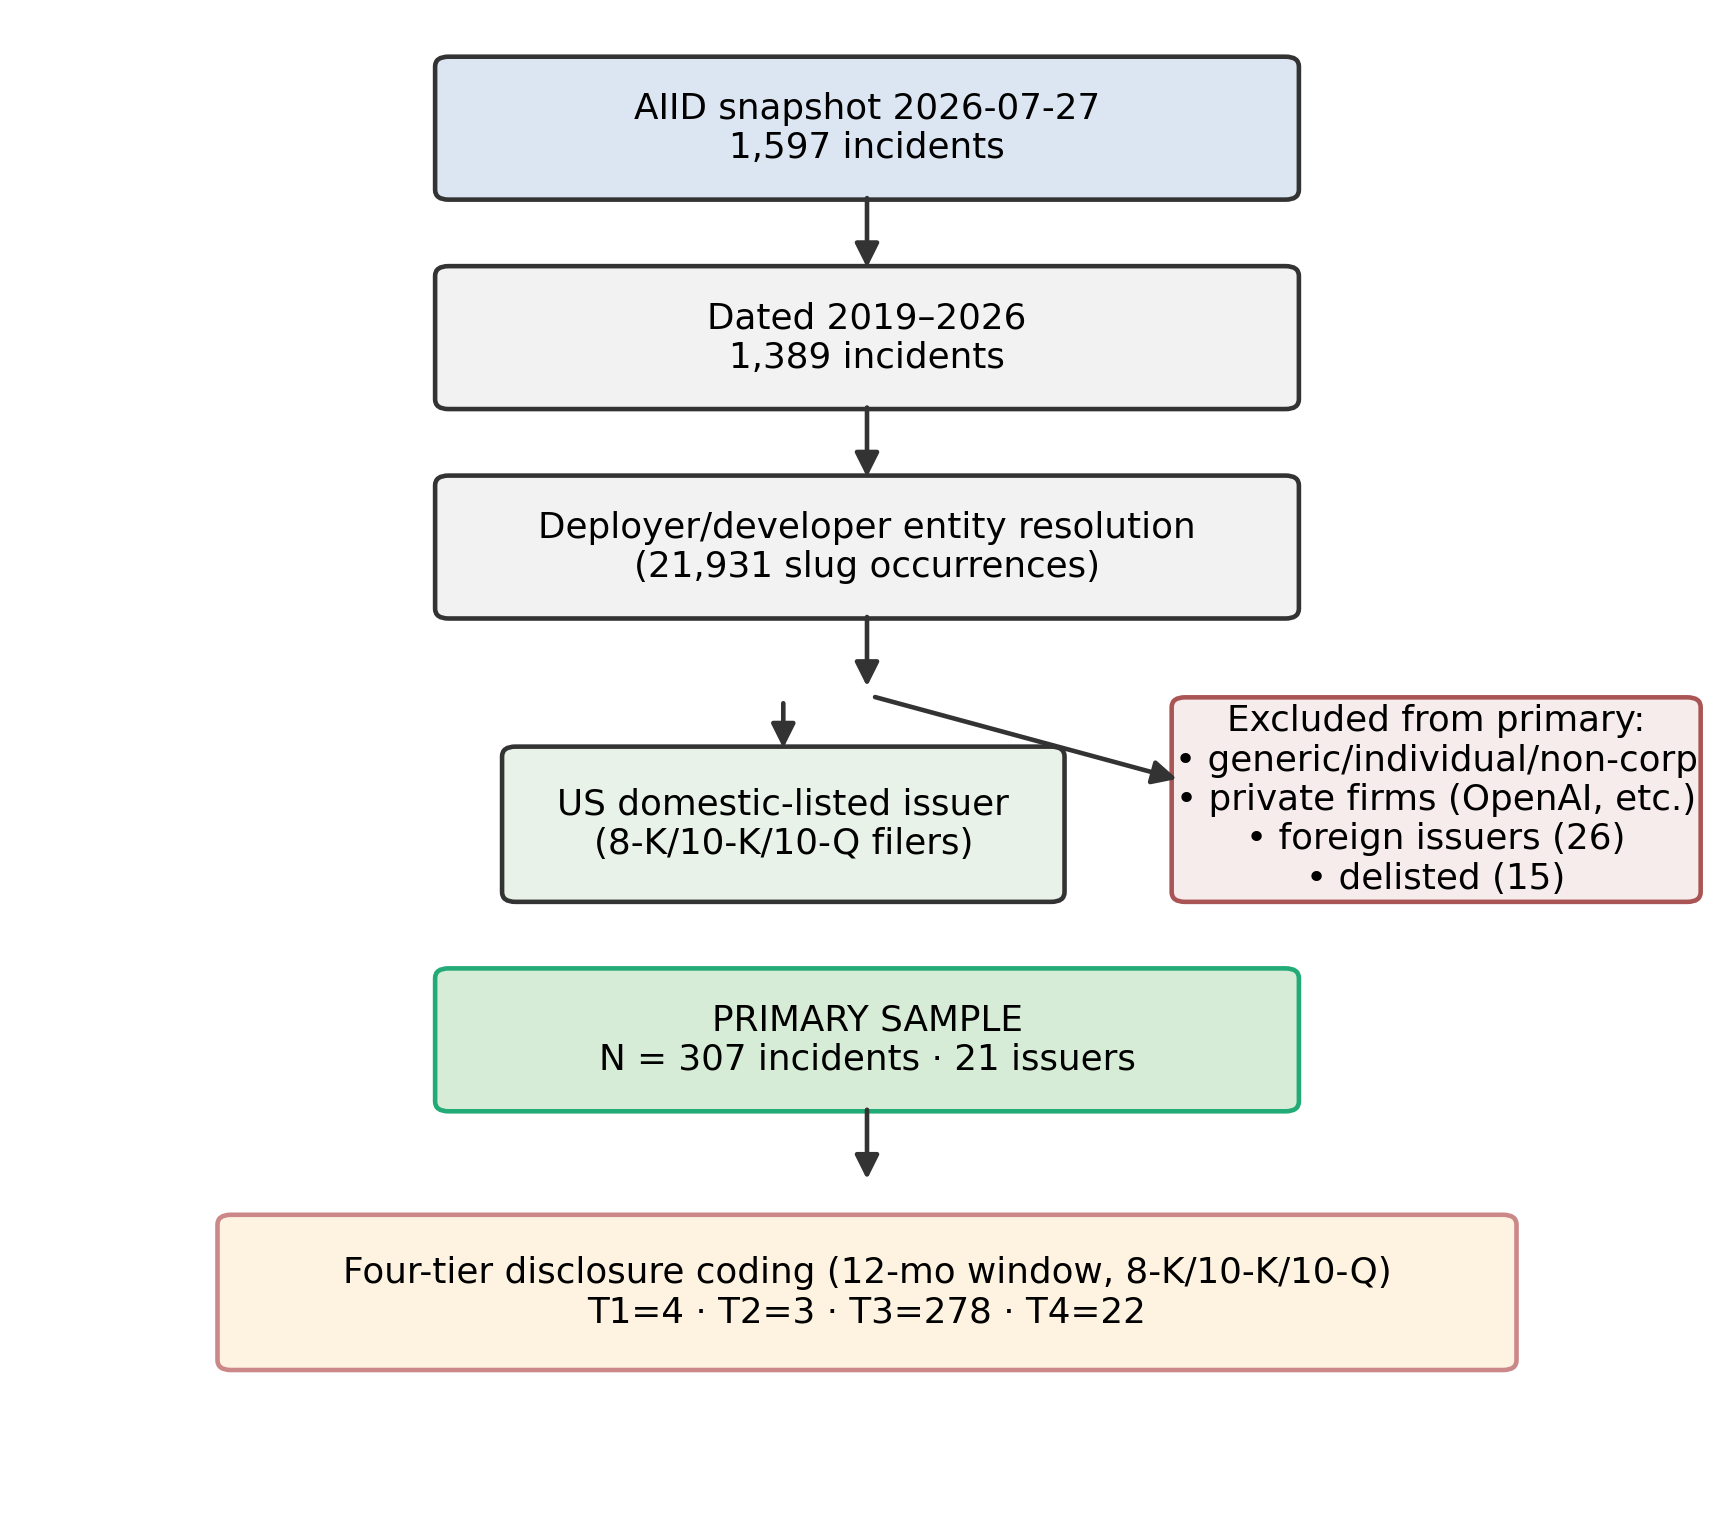
\includegraphics[width=0.82\textwidth]{figures/fig1.png}\end{center}
\caption{Sample construction: from 1{,}597 AIID incidents to the primary matchable population of N = 307 (21 issuers), with exclusion branches.}\label{fig:flow}
\end{figure}

\begin{figure}[h!]
\begin{center}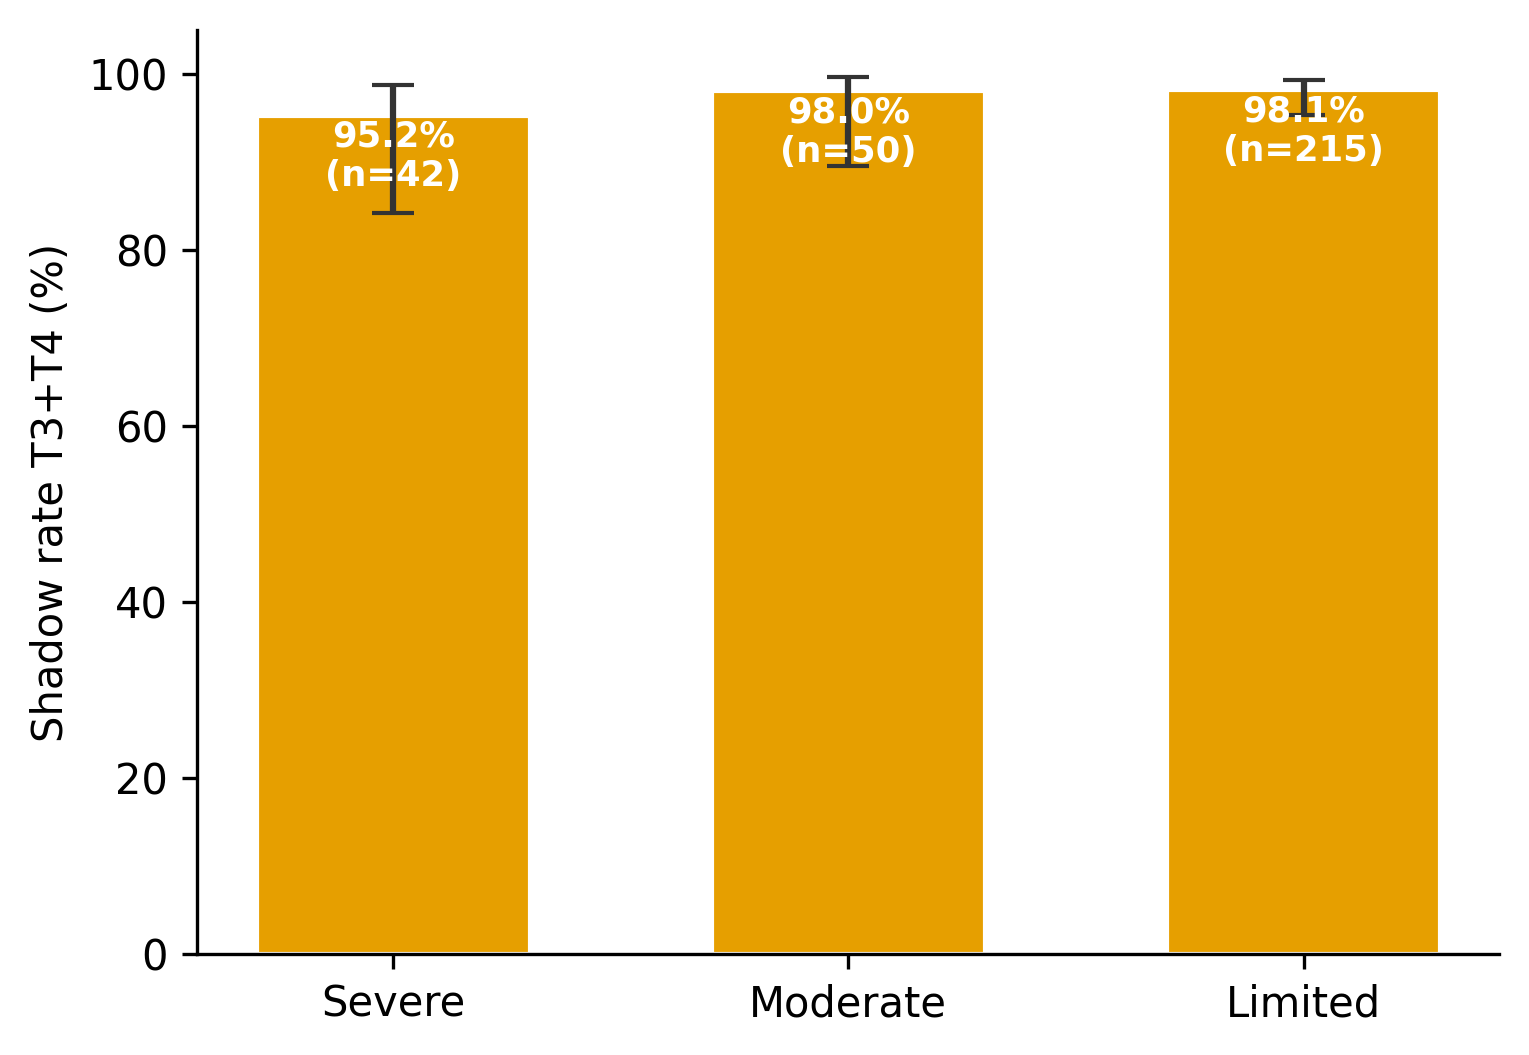
\includegraphics[width=0.62\textwidth]{figures/fig2.png}\end{center}
\caption{Shadow rate (T3+T4) by incident severity, with 95\% Wilson intervals.}\label{fig:sev}
\end{figure}

\begin{figure}[h!]
\begin{center}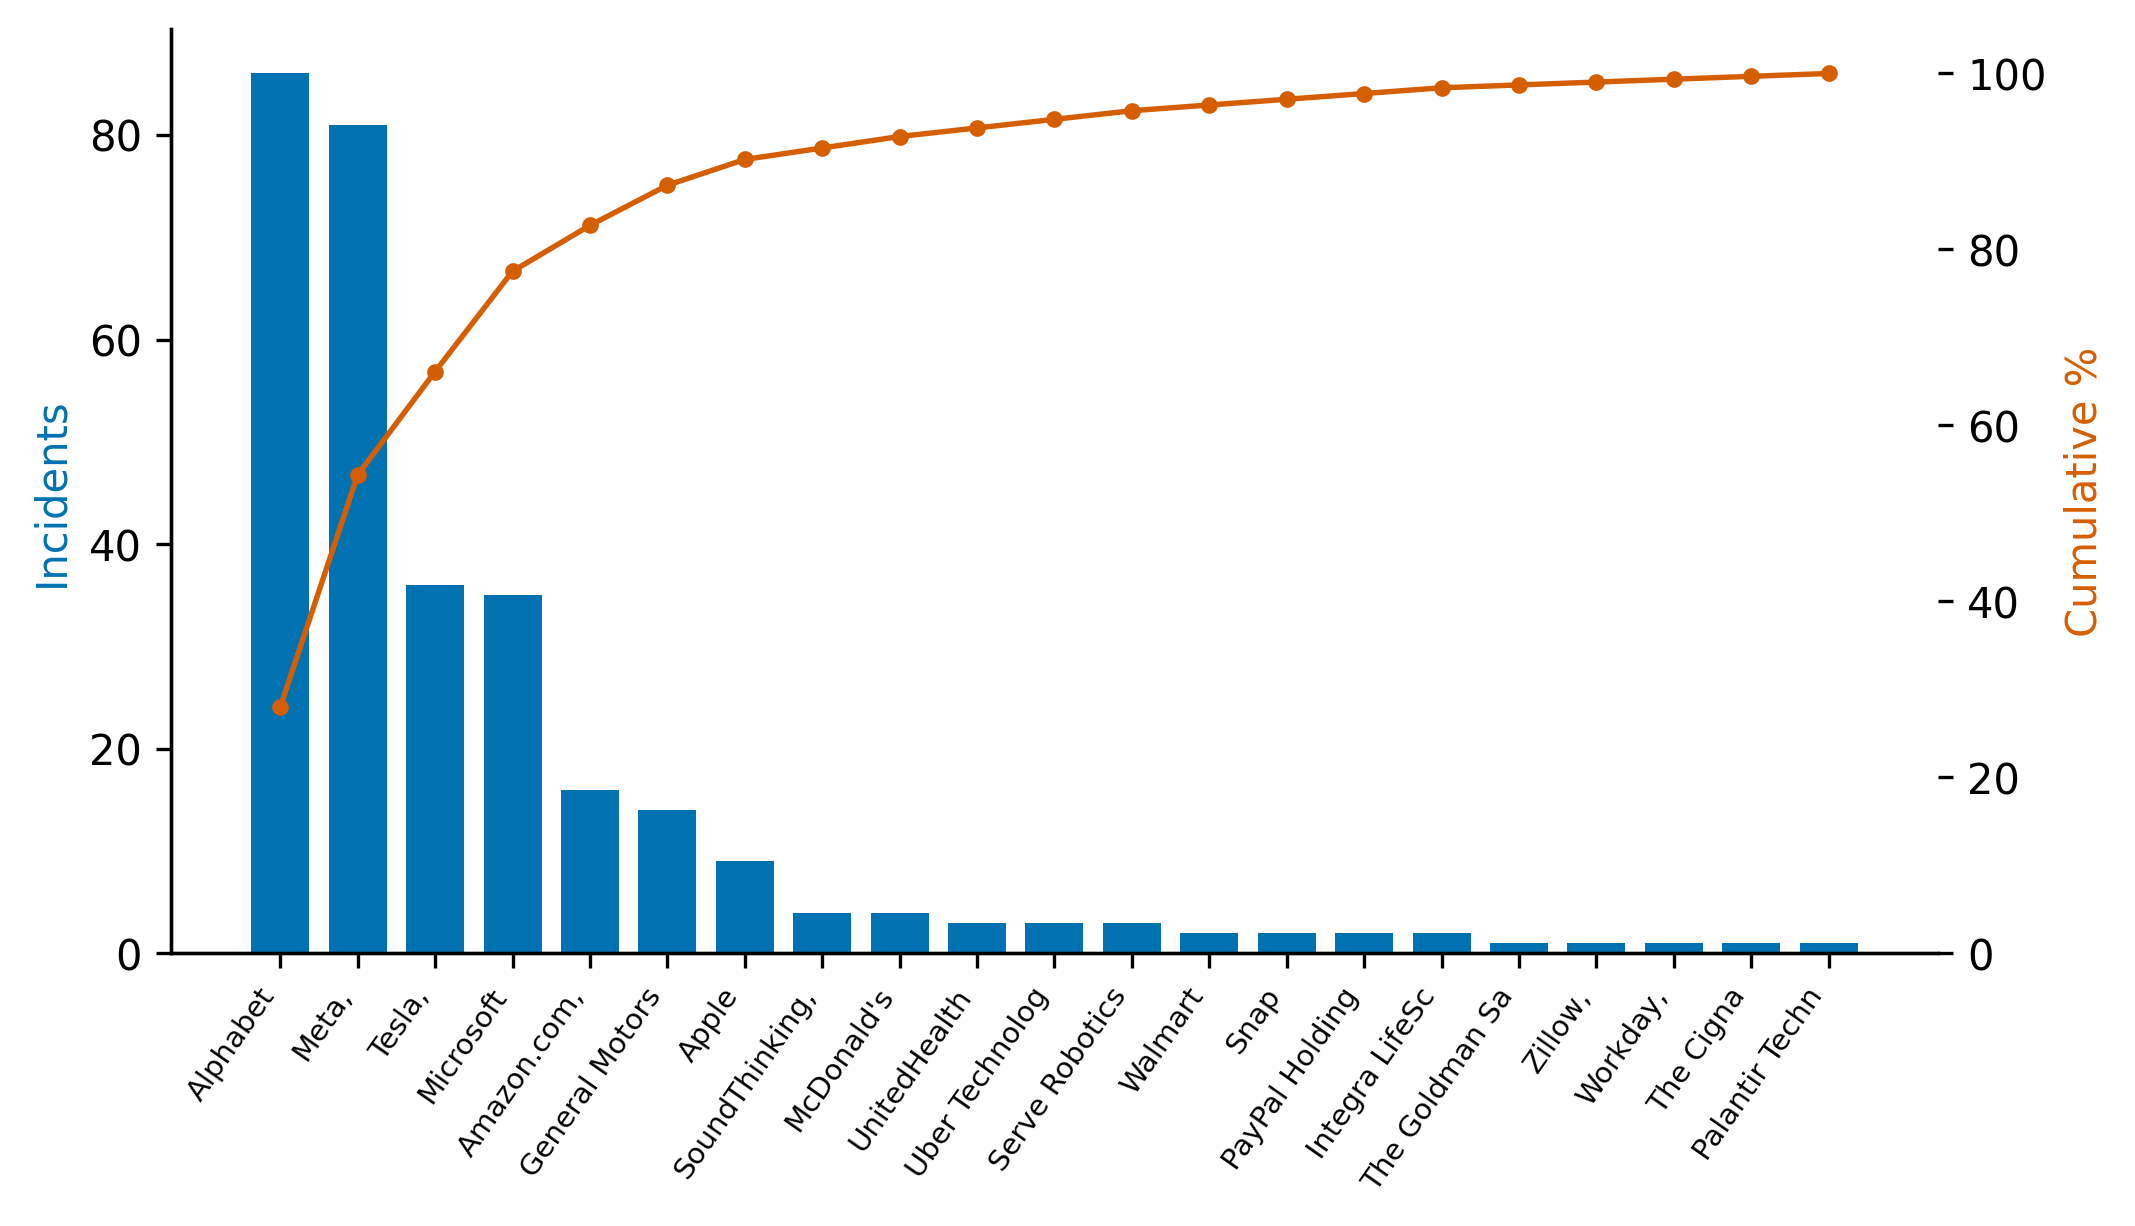
\includegraphics[width=0.9\textwidth]{figures/fig3.png}\end{center}
\caption{Incident concentration by issuer (Pareto): incidents per issuer and cumulative share.}\label{fig:pareto}
\end{figure}

\begin{figure}[h!]
\begin{center}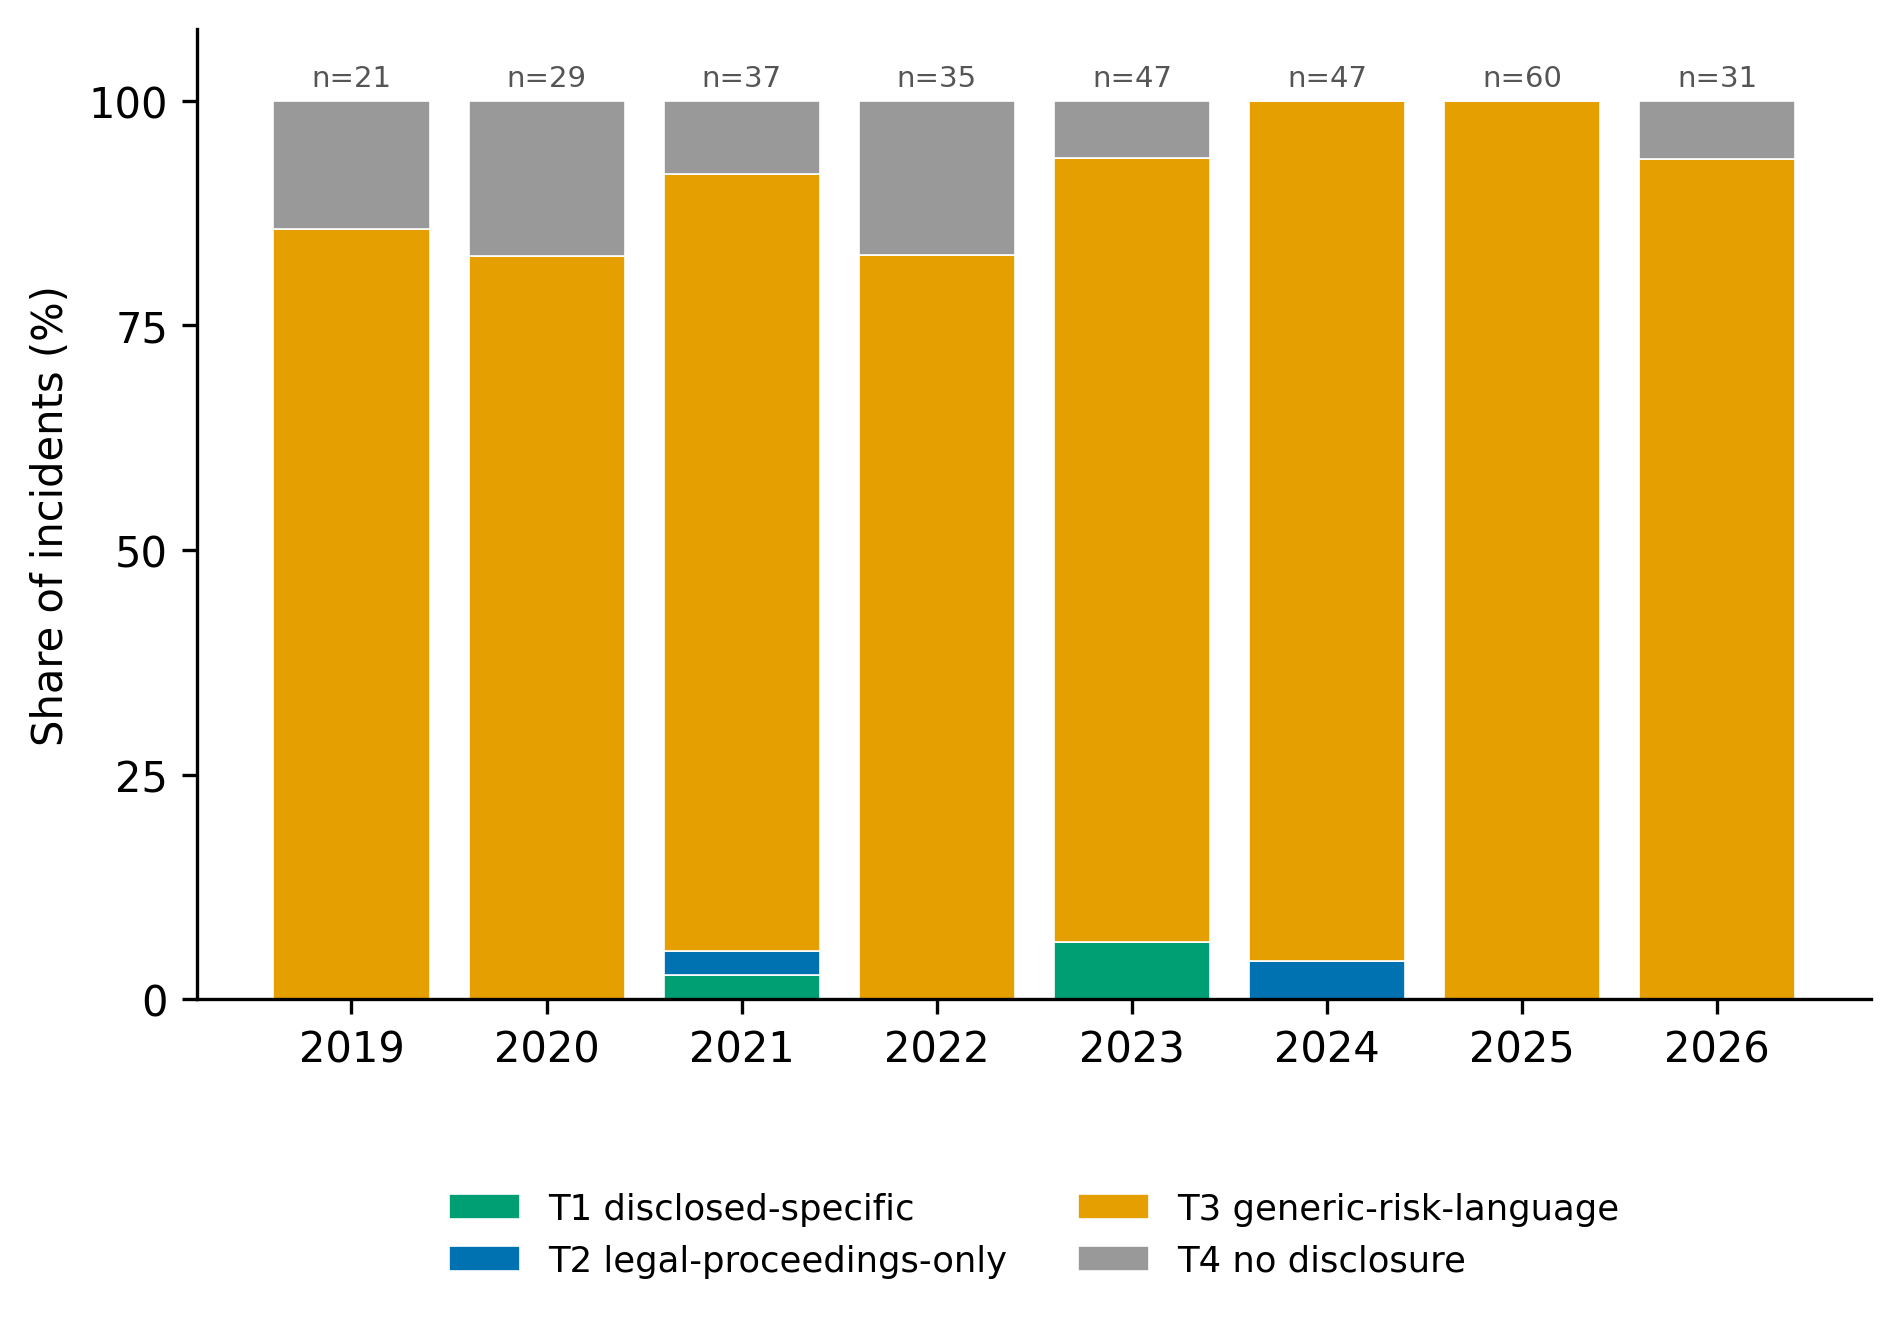
\includegraphics[width=0.9\textwidth]{figures/fig4.png}\end{center}
\caption{Disclosure tier by incident year (share of incidents).}\label{fig:year}
\end{figure}


\end{document}
